\chapter{The Church-Turing Thesis}

\lecture{8}{2025-11-10}{}

\section{Turing Machines}

\begin{prev}
    To discuss the \red{computability} of problems. We need a more powerful model. We already have seen
    \begin{itemize}
        \item Finite Automata (FA): with limited memory (states)
        \item Pushdown Automata (PDA): unlimited memory with LIFO structure (stack)
    \end{itemize}
\end{prev}

We now introduce a new computational model called \textbf{Turing Machine }(TM), which has an unlimited tape as memory.

\begin{figure}[H]
    \centering
    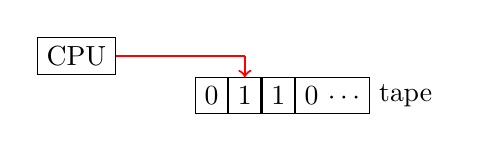
\begin{tikzpicture}[ampersand replacement=\&]
    \matrix 
    {
      \node[draw](0) {CPU}; \& [1cm] \& \node(1){}; \&\&\& \\
      \& \node[draw]{0}; \& \node[draw](a){1}; \& \node[draw]{1}; \& \node[draw]{0 $\cdots$};  \& \node{tape};\\
    };
    \draw [-,red,thick] (0) -- (1.center) ;
    \draw [->,red,thick] (1.center) -- (a) ;
    \end{tikzpicture}
    \caption{Illustration of a Turing Machine}
\end{figure}

A Turing Machine consists of these properties different from FA and PDA:
\begin{itemize}
    \item write/read tape
    \item head that can move left/right on the tape
    \item unlimited tape length
    \item reject/accept take immediate effect
    \item machine can \textbf{never} halt
\end{itemize}

\begin{eg}
    \[
        B = \{ w \# w \mid w \in \{0,1\}^* \}
    \]
\end{eg}
\begin{remark}
    We can proof that this language is not CFL by pumping lemma for CFL.
\end{remark}
\begin{notation}
    $\sqcup$ is the blank symbol on the tape.
\end{notation}

\newpage

\begin{idea}
    Zig-zag to the corresponding places on the two sides of the $\#$ and determine whether they match.
    \begin{itemize}
        \item Scan to check if ther is a $\#$.
        \item Check $w$ and $w$ if they match.
    \end{itemize}
\end{idea}

\begin{figure}[H]
    \centering
    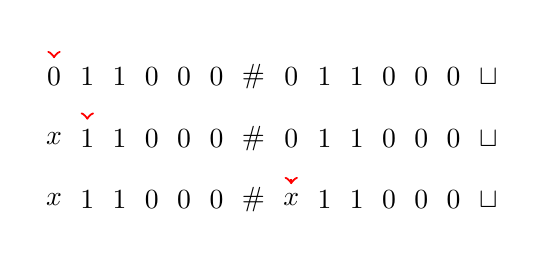
\begin{tikzpicture}[ampersand replacement=\&]
    \matrix 
    {
    \node(0){};  \&\&\&\&\&\& \& \&\&\&\&\&\& \\
    \node(01){0}; \& \node{1}; \& \node{1}; \& \node{0}; \& \node{0}; \&\node{0}; \&
    \node{\#}; \& 
    \node{0}; \& \node{1}; \& \node{1}; \& \node{0}; \& \node{0}; \& \node{0}; \& \node{$\sqcup$}; \\
        \& \node(1){};  \&\&\&\&\& \& \&\&\&\&\&\& \\
    \node{$x$}; \& \node(11){1}; \& \node{1}; \& \node{0}; \& \node{0}; \&\node{0}; \&
    \node{\#}; \& 
    \node{0}; \& \node{1}; \& \node{1}; \& \node{0}; \& \node{0}; \& \node{0}; \& \node{$\sqcup$}; \\
    \&\&\&\&\&\& \&    \node(2){};   \&\&\&\&\&\& \\
    \node{$x$}; \& \node{1}; \& \node{1}; \& \node{0}; \& \node{0}; \&\node{0}; \&
    \node{\#}; \& 
    \node(21){$x$}; \& \node{1}; \& \node{1}; \& \node{0}; \& \node{0}; \& \node{0}; \& \node{$\sqcup$}; \\
    };
    \draw [->,red,thick] (0) -- (01) ;
    \draw [->,red,thick] (1) -- (11) ;
    \draw [->,red,thick] (2) -- (21) ;
    % \draw [->,red,thick] (1.center) -- (a) ;
    \end{tikzpicture}
    \caption{Illustration of algorithm}
\end{figure}

\begin{definition}[Turing Machine (TM)]
    A Turing Machine is a 7-tuple \[
        M = (Q, \Sigma, \Gamma, \delta, q_0, q_\text{accept}, q_\text{reject})
    \]
    where
    \begin{itemize}
        \item \(Q\): States
        \item \(\Sigma\): Input alphabet, where \(\sqcup \notin \Sigma\)
        \item \(\Gamma\): Tape alphabet, where \(\Sigma \subset \Gamma\) and \(\sqcup \in \Gamma\)
        \item \(\delta\): Transition function
        \[
            \delta: Q \times \Gamma \to Q \times \Gamma \times \{L, R\}
        \]
        \item \(q_0 \in Q\): Start state
        \item \(q_\text{accept} \in Q\)
        \item \(q_\text{reject} \in Q, \ q_\text{reject} \neq q_\text{accept}\)
    \end{itemize}
\end{definition}

The input \[
    w = w_1 w_2 \cdots w_n \in \Sigma^*
\]
will be put in the position $1, 2, \cdots ,n$ of the tape, and the rest of the tape is filled with $\sqcup$.

\begin{eg}
    \[
        L = \{ 0^{2^n} \mid n \geq 0 \}
    \]
\end{eg}

\begin{idea}
    Cross off every second, and check if the remaining is even (except the last one).
    \begin{align*}
        & 0\underline{0} 0\underline{0}\\
        & 0\underline{0}\\
        & 0
    \end{align*}
\end{idea}

\newpage

The procedure should be:
\begin{enumerate}[label=$\arabic*^\circ$]
    \item left $\to$ right, make remark on every second 0
    \item if step $1^\circ$ left with only one unmarked 0, accept
    \item if step $1^\circ$ left with odd $\# 0$ left, reject 
    \item move head to the leftmost
    \item go to step $1^\circ$
\end{enumerate}

The definition of the machine is 
\begin{align*}
    Q &= \{ q_0, q_1, q_2, q_3, q_4, q_5, q_\text{accept}, q_\text{reject} \} \\
    \Sigma &= \{ 0 \} \\
    \Gamma &= \{ 0, x, \sqcup \} \\
\end{align*}
\begin{figure}[H]
    \centering
    \begin{tikzpicture}[node distance=2.5cm, ->, >=Stealth, on grid, auto]
    \node[state,initial above] (q_1) {$q_1$};
    \node[state] (q_2) [right of=q_1,xshift=0.5cm] {$q_2$};
    \node[state] (q_3) [right of=q_2,xshift=1.7cm] {$q_3$};
    \node[state] (q_4) [below of=q_3, yshift=0cm, xshift=0cm] {$q_4$};
    \node[state] (q_5) [above right of=q_2, yshift=0cm] {$q_5$};
    \node[state] (q_r) [below of=q_1, yshift=0cm] {$q_r$};
    \node[state] (q_a) [below of=q_2, yshift=0.7cm] {$q_a$};
    \path 
    (q_1) edge[below]  node {$0 \rightarrow \sqcup$, R} (q_2)
    (q_1) edge[right]  node {
    \begin{tabular}{l}
        $\sqcup \rightarrow$ R\\
        $x$   $ \rightarrow$ R\\
    \end{tabular}} (q_r)
    (q_2) edge[loop above]  node {$x$ $ \rightarrow $ R} (q_2)
    (q_2) edge[below]  node {$0 \rightarrow $ $x$, R} (q_3)
    (q_2) edge[right]  node {$\sqcup \rightarrow $ R} (q_a) 
    (q_3) edge[left, bend right=15]  node {$0 \rightarrow $ R} (q_4)
    (q_3) edge[loop right]  node {$x$ $ \rightarrow $ R} (q_3)
    (q_3) edge[right]  node {$\sqcup \rightarrow $ L} (q_5) 
    (q_4) edge[right, bend right=15]  node {$0 \rightarrow $ $x$, R} (q_3)
    (q_4) edge[loop right] node {$x$ $ \rightarrow $ R} (q_4)
    (q_4) edge[above, bend left=20]  node {$\sqcup \rightarrow $ R} (q_r)
    (q_5) edge[loop above]  node {
    \begin{tabular}{l}
        $0 \rightarrow $ L\\
        $x$ $\rightarrow$ L
    \end{tabular}
    } (q_5)
    (q_5) edge[right]  node {$\sqcup \rightarrow$ R } (q_2)    
    ;
  \end{tikzpicture}
    \caption{TM for \(L = \{ 0^{2^n} \mid n \geq 0 \}\)}
\end{figure}

\begin{notation}
    \[
        0 \to R \equiv 0 \to 0, R
    \]
\end{notation}

Consider the input \(0000\):
\begin{center}
    \begin{tabular}{lllll}
        $q_1 0000$ & $\sqcup q_2 000$ & $\sqcup x q_3 00$ & $\sqcup x 0 q_4 0$
        & $\sqcup x 0 x q_3$                                         \\
        $\sqcup x 0 q_5 x$ & $\sqcup x q_5 0 x$ & $\sqcup q_5 x 0 x$
        &  $q_5 \sqcup x 0 x$ & $\sqcup q_2  x 0 x$ \\
    $\sqcup x q_2  0 x$ & $\sqcup x x q_3  x$ & $\sqcup x x x q_3  \sqcup $
    & $\sqcup x x q_5 x $ & $\sqcup x q_5 x x $\\
    $\sqcup q_5 x x x $ & $q_5 \sqcup  x x x $ & $\sqcup  q_2 x x x $
    & $\sqcup  x q_2 x x $ & $\sqcup  x x q_2 x $ \\
    $\sqcup  x x x q_2$ & $\sqcup  x x x \sqcup q_a$ &&&
    \end{tabular}
\end{center}

The transition function table is as follows:
\begin{center}
    \begin{tabular}{c|ccc}
    & 0 & x & $\sqcup$\\ \hline
    $q_1 $ & $q_2,\sqcup,R$ & $q_{reject},x,R$ & $q_{reject},\sqcup,
    R$\\
    $q_2$ & $q_3,x,R$ & $q_2,x,R$ & $q_{accept},\sqcup,R$
    \\
    $\vdots$ &&&
    \end{tabular}
\end{center}

\newpage

\begin{note}
    There is no need for transition for \(q_\text{accept}\) and \(q_\text{reject}\) since the machine halts when it enters these states.
\end{note}

\begin{idea}
    We can get the design idea of Turing Machine
    \begin{itemize}
        \item $q_1: $ mark the start by $\sqcup$
        \begin{itemize}
            \item first element must be 0, otherwise, reject
            \item Using $\sqcup$, so the start is known
        \end{itemize}
        \item $q_2 \rightarrow q_3$: handle initial 00
        \item $q_3\rightarrow q_4 \rightarrow q_3$: sequentially $00 \rightarrow 0x$
        \begin{itemize}
            \item If not pairs (e.g., 0x0x0x), fails
            \item This is the place of checking if \# of remained zeros is even
        \end{itemize}
        \item $q_3 \rightarrow q_5 \rightarrow q_2 $ back to beginning
        \item first First 0 (or $\sqcup$) is considered the single final 0
        \[
            q_2 \rightarrow \cdots \rightarrow q_2 \rightarrow \cdots \rightarrow q_{accept}
        \]
        check if a single 0 is left in the string.
    \end{itemize}
\end{idea}

\subsection{Configuration of Turing Machine}

\begin{definition}[current configuration]
    The current configuration of a Turing Machine is represented as \[
        u q v
    \]
    where
    \begin{itemize}
        \item \(u \in \Gamma^*\): the string on the left of the head
        \item \(q \in Q\): the current state
        \item \(v \in \Gamma^*\): the string on the right of the head
    \end{itemize}
    The head is reading the first symbol of \(v\). If \(v = \epsilon\), then the head is reading a blank symbol \(\sqcup\).
\end{definition}

\begin{definition}
    $a, b, c \in \Gamma$, $u, v \in \Gamma^*,\ q_i, q_j \in Q$
    then the transition from configuration
    \begin{itemize}
        \item If \(\delta(q_i, b) = (q_j, c, L)\), then
        \[
            u a q_i b v \vdash u q_j a c v
        \]
        \item If \(\delta(q_i, a) = (q_j, b, L)\), then
        \[
            u a q_i b v \vdash u a c q_j v
        \]
    \end{itemize}
\end{definition}

\newpage

\subsection{Turing Recognizable and Turing Decidable Languages}

\begin{definition}[Turing Recognizable]
    A language \(L\) is Turing recognizable if some Turing Machine \(M\) recognizes it.
\end{definition}

For a Turing Machine there are three possible outcomes:
\begin{itemize}
    \item Accept the input by entering \(q_\text{accept}\)
    \item Reject the input by entering \(q_\text{reject}\)
    \item Loop forever without halting
\end{itemize}

A language is very difficult to difficult to decide if the TM loops forever on some inputs. We now define a more restricted type of model, called \textbf{Decider}.

\begin{definition}[Turing Decidable]
    A language \(L\) is Turing decidable if some Turing Machine \(M\) decides it.
\end{definition}

We will discuss more about Decidability in later chapters (Ch.4).

\subsection{Example of Turing Machine}

\begin{eg}
    \(
        L = \{ w\#w \mid w \in \{0,1\}^* \}
    \)
\end{eg}

\begin{figure}[H]
    \centering
    \begin{tikzpicture}[>=Stealth, ->, auto, every loop/.style={min distance=10mm}]
        \node[state,initial above] (q_1) at (0,1.8) {$q_1$};
        \node[state] (q_2) at (-4,0) {$q_2$};
        \node[state] (q_8) at (0,0) {$q_8$};
        \node[state] (q_3) at (4,0) {$q_3$};
        \node[state] (q_4) at (-4,-2.8) {$q_4$};
        \node[state] (q_a) at (0,-2.8) {$q_a$};
        \node[state] (q_5) at (4,-2.8) {$q_5$};
        \node[state] (q_7) at (-4,-5.6) {$q_7$};
        \node[state] (q_6) at (0,-5.6) {$q_6$};
        \path 
        (q_1) edge[above] node {$0 \rightarrow x, R$} (q_2)
        (q_1) edge[right]  node {$\# \rightarrow R$} (q_8)
        (q_1) edge[right] node {$1 \rightarrow x, R$} (q_3) 
        (q_2) edge[loop left]  node {$0,1 \rightarrow R$} (q_2)
        (q_2) edge[left]  node {$\# \rightarrow R$} (q_4)  
        (q_8) edge[loop right]  node {$x \rightarrow R$} (q_8)
        (q_8) edge[right]  node {$\sqcup \rightarrow R$} (q_a)
        (q_3) edge[loop right]  node {$0,1 \rightarrow R$} (q_3)
        (q_3) edge[right]  node {$\# \rightarrow R$} (q_5)
        (q_4) edge[loop below]  node {$x \rightarrow R$} (q_4)
        (q_4) edge[bend right=15]  node[left] {$0 \rightarrow x, L$} (q_6)
        (q_5) edge[loop below]  node {$x \rightarrow R$} (q_5)
        (q_5) edge[bend left=15]  node[right] {$1 \rightarrow x, L$} (q_6)
        (q_6) edge[loop below]  node {$0,1,x \rightarrow L$} (q_6)
        (q_6) edge[below]  node {$\# \rightarrow L$} (q_7)
        (q_7) edge[loop left]  node {$0,1 \rightarrow L$} (q_7)
        (q_7) edge node {$x \rightarrow R$} (q_1);    
    \end{tikzpicture}
    \caption{Turing Machine of \(L = \{ w\#w \mid w \in \{0,1\}^* \}\)}
\end{figure}

\begin{remark}
    Links to \(q_r\) are not shown
\end{remark}

\newpage

Simulate $01\#01$

\begin{center}
\begin{tabular}{llll}
  $q_1 0 1 \# 01$ & $x q_2 1 \# 01$ & $x1 q_2 \# 01$ & $x1\# q_4 01$
  \\
  $x1 q_6 \# x 1$ & $x q_7 1 \# x 1$ & $ q_7 x 1 \# x 1$ & $x q_1 1 \# x 1$
  \\
  $xx q_3 \# x 1$ & $xx \# q_5 x 1$ & $xx \# x q_5 1$ & $xx \# q_6 xx$ \\
  $xx q_6 \# xx$ & $x q_7 x \# xx$ & $xx q_1 \# xx$ & $xx \# q_8 xx$ \\
 $xx \# xx q_8 \sqcup$ &  $xx \# xx \sqcup q_a$ &&
\end{tabular}
\end{center}

\begin{idea}
The diagram:
  \begin{equation*}
    q_1 \rightarrow q_2 \rightarrow q_4 \rightarrow q_6
  \end{equation*}
  check 0 at the same position of the two strings
  \begin{equation*}
    q_1 \rightarrow q_3 \rightarrow q_5 \rightarrow q_6    
  \end{equation*}
  check 1 at the same position of the two strings
\end{idea}

\begin{eg}
    \(
        C = \{ a^i b^j c^k \mid i \times j = k, \ i,j,k \geq 1 \}
    \)
\end{eg}

\begin{idea}
    The procedure should be:
    \begin{enumerate}[label=$\arabic*^\circ$]
        \item check if the input is $a^+b^+c^+$
        \item back to the leftmost $a$
        \item fix an $a$, for each $b$, cross off a $c$
        \item store $b$ back, cancel one $a$, repeat step 3
    \end{enumerate}
\end{idea}

\begin{itemize}
    \item Step 1 can be done by a DFA (as DFA is a special case of TM).
    \item Step 2 can be done by moving left until $\sqcup$ is reached.
    \item Step 3 is similar to previous examples.
\end{itemize}

\begin{eg}
    \(
        E = \{ \# x_1 \# x_2 \cdots \# x_l \mid x_i \in \{0,1\}^*, \ x_i \neq x_j \}
    \)
\end{eg}

\begin{idea}
    Sequentially compare every pairs
    \begin{equation*}
    \begin{split}
    & x_1 x_2, x_1 x_3, \ldots, x_1 x_l \\
    & x_2 x_3, \ldots, x_2 x_l \\
    & \vdots \\
    & x_{l-1} x_l
    \end{split}
    \end{equation*}
    For $x_i,\ x_j$, mark $\#$'s strings by $\dot{\#}$ i.e.
    \[
        \dot{\#}x_1\#x_2 \dot{\#}x_3: x_1 \text{ and } x_3 \text{ are compared}
    \]
    We can copy $x_i$, $x_j$ to the right end of the tape and compare them there with the pattern of $w\#w$.
\end{idea}


